\ifslide{

  \section{Agenda}
  \begin{frame}{Agenda}
    \begin{block}{Session outline}
      \begin{itemize}
        \item how to use an IDE (Eclipse)
        \item control structure (if, for, while, .switch,...)
        \item functions
        \item error handling
      \end{itemize}
    \end{block}
  \end{frame}

  \section{Using an IDE: Eclipse}

  \begin{frame}{What is an Integrated Development Environment ?}
    \begin{block}{Main features}
      \begin{itemize}
        \item Advanced file editing
        \begin{itemize}
          \item highlight syntax with colors
          \item syntax checker
          \item auto completion
        \end{itemize}
        \item Program building
        \begin{itemize}
          \item compilation
          \item run program inside the IDE
        \end{itemize}
        \item \textbf{debugger}
        \begin{itemize}
          \item execute program \textbf{interactively}
          \item expose variables content, allow to modify them direclty
        \end{itemize}
      \end{itemize}
    \end{block}
  \end{frame}
}

\ifslide{
  \begin{frame}{A short Eclipse Tutorial}
    \begin{block}{Eclipse IDE}
      \begin{itemize}
        \item Open Source, java based, IDE
        \item Most used IDE in the World
        \item Focus on Java programming but also used for other technologies
        \item Cross platform program
        \item Speed up development (up to 40\% !)
      \end{itemize}
    \end{block}
  \end{frame}


  \begin{frame}{Use Eclipse (1/2)}
    \begin{block}{Instructions}
      \begin{itemize}
        \item Look for Eclipse in the Application launcher menu, and start it
        \item Eclipse will ask for the location of the \textbf{workspace}
        \begin{itemize}
          \item this location is where Eclipse stores the project's files
          \item simply click on "OK" and accept the default location
        \end{itemize}
        \item Go to File->New->Java Project to create a new, empty, Java project.
        \item Use your first and lastname (ex:romain-pelisse) as project name and click sur "Finish"
        \item \textbf{Right-click} on the folder 'src' and select the 'import' options:
        \begin{itemize}
          \item a wizard will appear to specifify the import method
          \item select General->File System and click on "Next"
          \item use the "Browser" button to select the "Desktop" folder
          \item select all the java sources files (.java) on Deskopt (all files from the previous
          session)
          \item click on "Finish" to import all of them
        \end{itemize}
      \end{itemize}
    \end{block}
  \end{frame}

  \begin{frame}{Use Eclipse (2/2)}
    \begin{block}{Instructions}
      \begin{itemize}
        \item Compile, run and \textbf{debug}:
        \begin{itemize}
          \item Eclipse will compile for you, automatically any Java files in the src/ folder -
          nothing to do !
          \item To run a Java file, right-click on the file and select Run as->Java Application
          \item To Debug a program, right-click on the file and select Debug as->Java Application
        \end{itemize}
      \end{itemize}
    \end{block}
  \end{frame}
}

\ifslide {
  \begin{frame}{Use Eclipse's debugger}
    \begin{block}{Instructions}
      \begin{itemize}
        \item Double click on the column on the left of the source code to set a \textbf{breakpoint} - see picture below
        \item Run the program with the debugger (Debug as->Java Application) and ...
        \begin{itemize}
          \item run the program step-by-step
          \item examine the values of each available variables
          \item set a breakpoint and execute the program up to it
        \end{itemize}
      \end{itemize}
    \end{block}
  \end{frame}

   \section{Control Structure}

   \begin{frame}{The 'if' statement}
     \begin{block}{The 'if' statement}
      \begin{itemize}
        \item simple form of control flow statement.
        \item directs the program to execute a certain section of code...
        \item ...if and only if the test evaluates to true
        \item in Java, a the test must be boolean expression.
       \end{itemize}
     \end{block}

     \begin{block}{Instructions}
       \begin{itemize}
         \item Download the HowToUseIfStmt.java file and save it on the Desktop
         \item Import the file in your project as you did before
         \item Implements the program as defined in the source file
         \item To add an 'if' statement to the code, use the autocompletion feature of Eclipse
         (crtl+space)
       \end{itemize}
     \end{block}
   \end{frame}

}

\ifslide{
   \begin{frame}{The 'for' statement}
     \begin{block}{The 'for' statement}
      \begin{itemize}
        \item execute a block of code continuously
        \item consists of tree parts :\tiny{
        \begin{description}
          \item[initialization]: an expression that sets the value of the loop control variable,
          executed only once.
          \item[condition]:  a boolean expression that tests the loop control variable against a target
          value and hence works as a loop terminator.
          \item[Increment/decrement]: an expression that increments or decrements the loop
          control variable.
        \end{description}
        }
       \end{itemize}
     \end{block}

     \begin{block}{Instructions}
       \begin{itemize}
         \item Using Eclipse, copy the file HowToUseIfStmt.java to HowToUseForLoop.java
         \item This new program accepts only one character values as arguments:\texttt{java
         HowToUseForLoop 1 2 3 4 5 6 7} - there no more bound for the number of arguments.
         \item Modify the program accordingly
         \item To add a 'for' statement to the code, use the autocompletion feature of Eclipse
         (crtl+space)
       \end{itemize}
     \end{block}
   \end{frame}

   \begin{frame}{The 'while' statement}
     \begin{block}{The 'while' statement}
       \begin{itemize}
         \item execute a block of code continuously...
         \item ... as long as the condition is true.
         \item mix between an 'if' and a 'while'
         \item a \mylink{http://www.roseindia.net/java/beginners/DoWhile.shtml}{do...while} statement also exist - to skip the first evaluation.
       \end{itemize}
     \end{block}

     \begin{block}{Instructions}
       \begin{itemize}
         \item Download the file WhyWhileStmtAreAlsoCool.java
         \item Modify the program as requested in the code
       \end{itemize}
     \end{block}
   \end{frame}
}

\ifslide{
   \begin{frame}{The 'switch' statement}
     \begin{block}{The 'switch' statement}
      \begin{itemize}
        \item an alternative to a series of 'else if'
        \item allows for any number of possible execution paths
        \item works with the byte, short, char, and int primitive data types
        \item works with enumerated types (we'll see them later)
        \item body of a switch statement is known as a switch block.
        \item Any statement immediately contained by the switch block may be labeled:
        \begin{itemize}
          \item with one label
          \item several lables
          \item or the default label
        \end{itemize}
      \end{itemize}
     \end{block}

     \begin{block}{Remarks}
       \begin{itemize}
         \item powerful but rather complex
         \item seldom used
         \item generally just to remove a messy, long if statement
       \end{itemize}
     \end{block}
   \end{frame}
}

\section{Functions}

\ifslide{
  \begin{frame}
    \begin{block}{What is function ?}
       \textit{In computer science, a subroutine, also termed procedure, function, routine, method, or
       subprogram, is a part of source code within a larger computer program that performs a specific
       task and is relatively independent of the remaining code. - Wikipedia
       \mylink{http://en.wikipedia.org/wiki/Subroutine}{"Subroutine"}, accessed
       the 22.05.2012}
    \end{block}

    \begin{block}{What are their purpose ?}
      \begin{itemize}
        \item reuse code easily
        \item make code easier to read
        \item breakdown code in different, meaningful, part
        \item hide complexity
      \end{itemize}
    \end{block}
  \end{frame}

  \begin{frame}
    \begin{block}{Functions syntax}
      \begin{center}
        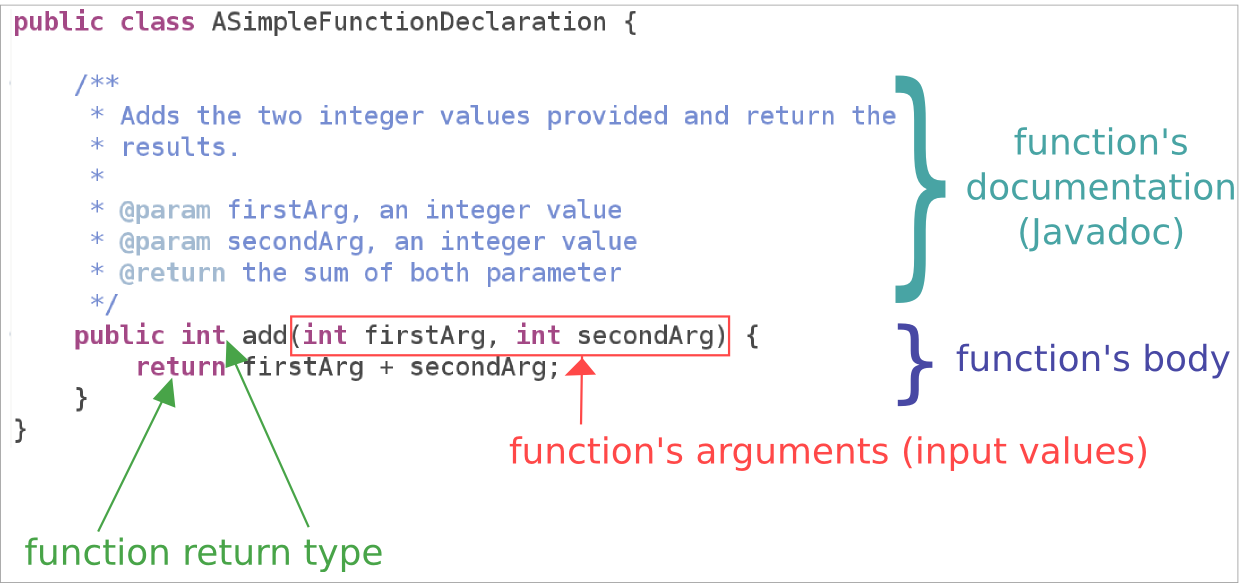
\includegraphics[scale=0.2]{../img/a-simple-java-function.png}
      \end{center}
    \end{block}

    \begin{block}{Instructions}
      \begin{itemize}
        \item Download and import the file called LenghtyProgram
        \item Modify the code according to the instruction
      \end{itemize}
    \end{block}
  \end{frame}
}

\section{Error Handling}
\ifslide{
 \begin{frame}
    \begin{block}{Structure to handle error in programming language}
      \begin{itemize}
        \item do nothing
        \begin{itemize}
          \item program crashes
          \item no information on the root cause
        \end{itemize}
        \item use "status code"
        \begin{itemize}
          \item functions can't return value
          \item leads to message such as "Error 400 happened"
          \item needs to have an error database to translate the status code
        \end{itemize}
        \item return a complete structure describing in length the error
        \begin{itemize}
          \item ideal, but...
          \item ...still remove the option of having returning value
        \end{itemize}
      \end{itemize}
    \end{block}
 \end{frame}
}
